\documentclass[tikz,border=2pt]{standalone}
\usepackage[T1]{fontenc}
\usepackage{mathptmx}
\usetikzlibrary{patterns,arrows.meta,calc}
\begin{document}
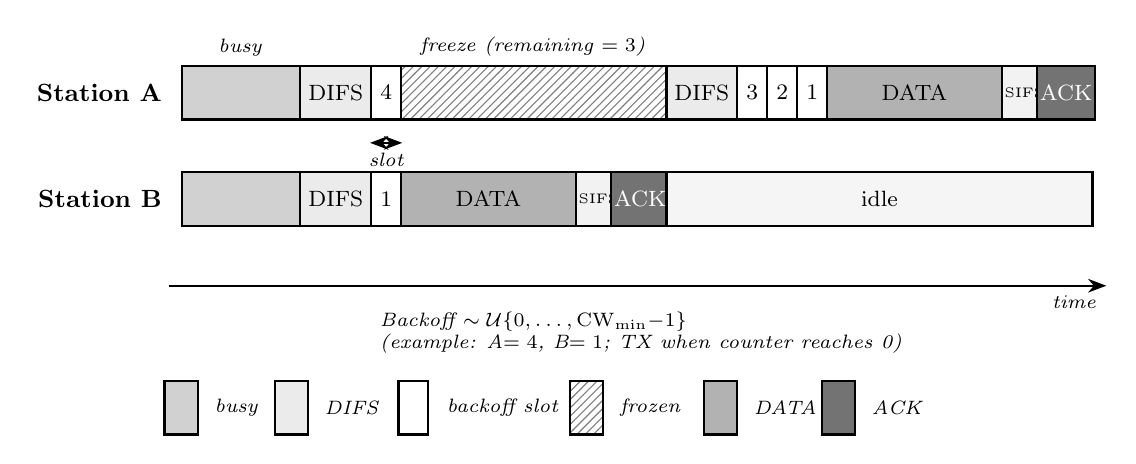
\begin{tikzpicture}[
  x=1cm,
  y=1cm,
  font=\footnotesize,
  >=Stealth,
  every node/.style={font=\footnotesize},
  bar/.style={draw, thick, minimum height=0.68cm, inner sep=1pt, align=center},
  busy/.style={bar, fill=black!18},
  difs/.style={bar, fill=black!8},
  slot/.style={bar, fill=white, minimum width=0.38cm},
  data/.style={bar, fill=black!30},
  ack/.style={bar, fill=black!55, text=white},
  freeze/.style={bar, pattern=north east lines, pattern color=black!50},
  sifs/.style={bar, fill=black!5},
  idle/.style={bar, fill=black!4},
  lbl/.style={font=\scriptsize\itshape},
]
  % Rule: a box labeled k is one idle slot while the counter equals k.
  % After that slot the counter becomes k-1; when it would reach 0, the
  % station transmits (DATA). So BO=1 → one box ``1'' then DATA;
  % remaining 3 → boxes ``3'',``2'',``1'' then DATA.
  \def\yA{2.50}
  \def\yB{1.15}
  \def\yAxis{0.05}
  \def\xoff{1.85}

  \node[anchor=east, font=\small\bfseries] at ({\xoff-0.12},\yA) {Station A};
  \node[anchor=east, font=\small\bfseries] at ({\xoff-0.12},\yB) {Station B};

  % Busy
  \node[busy, minimum width=1.5cm, anchor=west] at (\xoff,\yA) {};
  \node[busy, minimum width=1.5cm, anchor=west] at (\xoff,\yB) {};
  \node[lbl, above] at ({\xoff+0.75},\yA+0.34) {busy};

  % DIFS
  \node[difs, minimum width=0.9cm, anchor=west] at ({\xoff+1.5},\yA) {DIFS};
  \node[difs, minimum width=0.9cm, anchor=west] at ({\xoff+1.5},\yB) {DIFS};

  % Shared first idle slot: A=4, B=1 → after this slot A=3, B=0 → B transmits
  \node[slot, anchor=west] (a4) at ({\xoff+2.4},\yA) {4};
  \node[slot, anchor=west] (b1) at ({\xoff+2.4},\yB) {1};

  % B wins (counter reached 0); A freezes with remaining 3
  % [2.78–6.15] = DATA(2.22) + SIFS(0.45) + ACK(0.70)
  \node[data, minimum width=2.22cm, anchor=west] at ({\xoff+2.78},\yB) {DATA};
  \node[sifs, minimum width=0.45cm, anchor=west] at ({\xoff+5.0},\yB) {\tiny SIFS};
  \node[ack,  minimum width=0.70cm, anchor=west] at ({\xoff+5.45},\yB) {ACK};
  \node[freeze, minimum width=3.37cm, anchor=west] at ({\xoff+2.78},\yA) {};
  \node[lbl, above] at ({\xoff+4.465},\yA+0.34) {freeze (remaining $=3$)};

  % A resumes: DIFS + three idle slots (3,2,1) then DATA
  \node[difs, minimum width=0.9cm, anchor=west] at ({\xoff+6.15},\yA) {DIFS};
  \node[slot, anchor=west] at ({\xoff+7.05},\yA) {3};
  \node[slot, anchor=west] at ({\xoff+7.43},\yA) {2};
  \node[slot, anchor=west] at ({\xoff+7.81},\yA) {1};

  \node[data, minimum width=2.22cm, anchor=west] at ({\xoff+8.19},\yA) {DATA};
  \node[sifs, minimum width=0.45cm, anchor=west] at ({\xoff+10.41},\yA) {\tiny SIFS};
  \node[ack,  minimum width=0.70cm, anchor=west] at ({\xoff+10.86},\yA) {ACK};

  % B idle while A finishes (from 6.15 to end of A's ACK = 10.86+0.70 = 11.56)
  \node[idle, minimum width=5.41cm, anchor=west] at ({\xoff+6.15},\yB) {idle};

  \draw[<->, thick] ([yshift=-8pt]a4.south west) -- ([yshift=-8pt]a4.south east)
    node[midway, below, lbl] {slot};
  \node[lbl, anchor=west, align=left] at ({\xoff+2.4},-0.55) {%
    Backoff $\sim\mathcal{U}\{0,\ldots,\mathrm{CW}_{\min}{-}1\}$\\
    (example: A$=4$, B$=1$; TX when counter reaches 0)};

  \draw[->, thick] ({\xoff-0.15},\yAxis) -- ({\xoff+11.75},\yAxis)
    node[below left, lbl] {time};

  \begin{scope}[shift={({\xoff},-1.50)}]
    \node[busy, minimum width=0.42cm] at (0,0) {};
    \node[anchor=west, lbl] at (0.30,0) {busy};
    \node[difs, minimum width=0.42cm] at (1.4,0) {};
    \node[anchor=west, lbl] at (1.70,0) {DIFS};
    \node[slot] at (2.95,0) {};
    \node[anchor=west, lbl] at (3.25,0) {backoff slot};
    \node[freeze, minimum width=0.42cm] at (5.15,0) {};
    \node[anchor=west, lbl] at (5.45,0) {frozen};
    \node[data, minimum width=0.42cm] at (6.85,0) {};
    \node[anchor=west, lbl] at (7.15,0) {DATA};
    \node[ack, minimum width=0.42cm] at (8.35,0) {};
    \node[anchor=west, lbl] at (8.65,0) {ACK};
  \end{scope}
\end{tikzpicture}
\end{document}
